%Master File:lectures.tex

\lesson{Use Arrays}

\vspace*{-2cm}
\begin{center}
  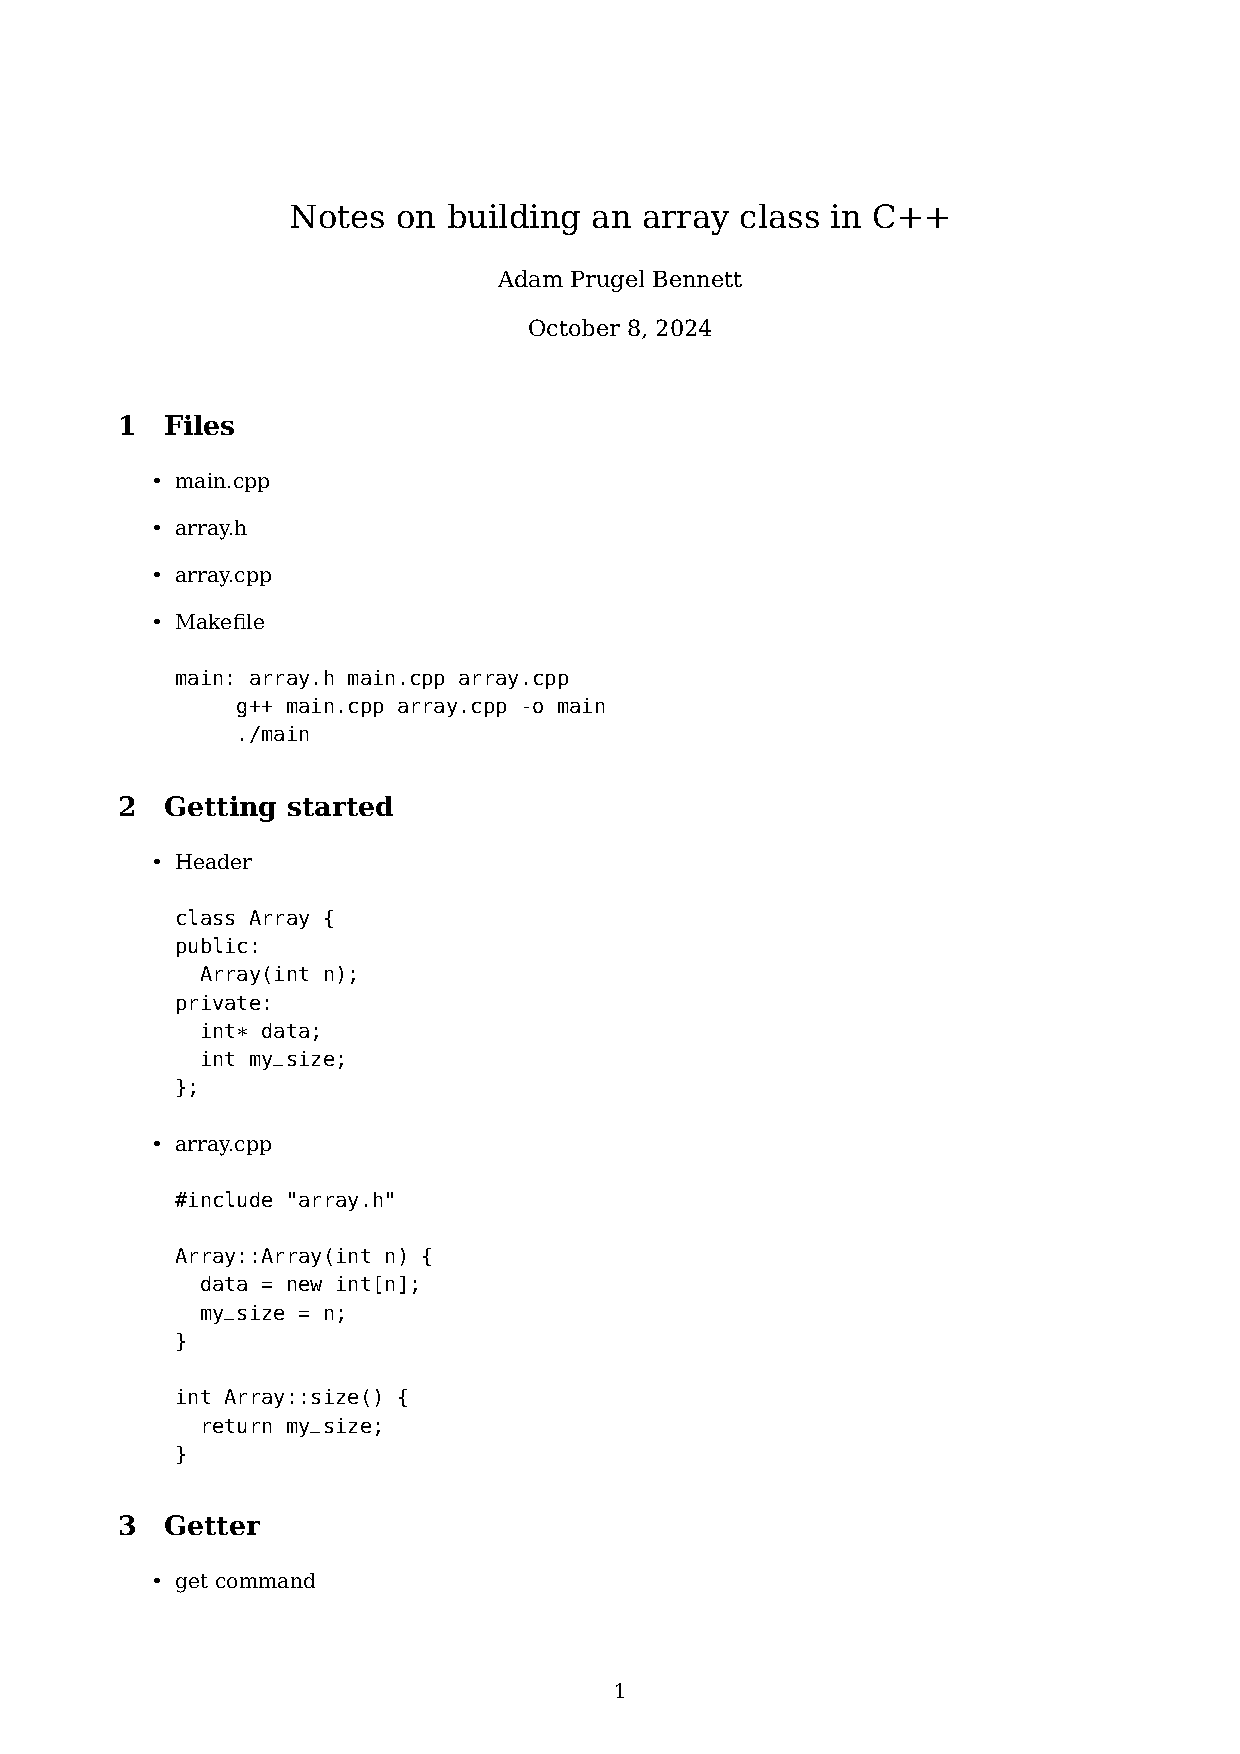
\includegraphics[height=11cm]{array}
\end{center}
\vspace*{-1cm}
\keywords{Variable length arrays, implementing stacks}

%%%%%%%%%%%%%%%%%%%%%%% Next Slide %%%%%%%%%%%%%%%%%%%%%%%

\renewcommand{\Outline}{%
\begin{slide}
\section{Outline}
\begin{minipage}{10cm}
  \vfill
  \begin{enumerate}
    \outlineitem{Why Arrays?}{intro}
    \outlineitem{Variable Length Arrays}{var}
    \outlineitem{Programming Language}{varimpl}
    \outlineitem{Implementing Stacks}{impl}
  \end{enumerate}
  \vfill
\end{minipage}\hfill
\begin{minipage}{10cm}
  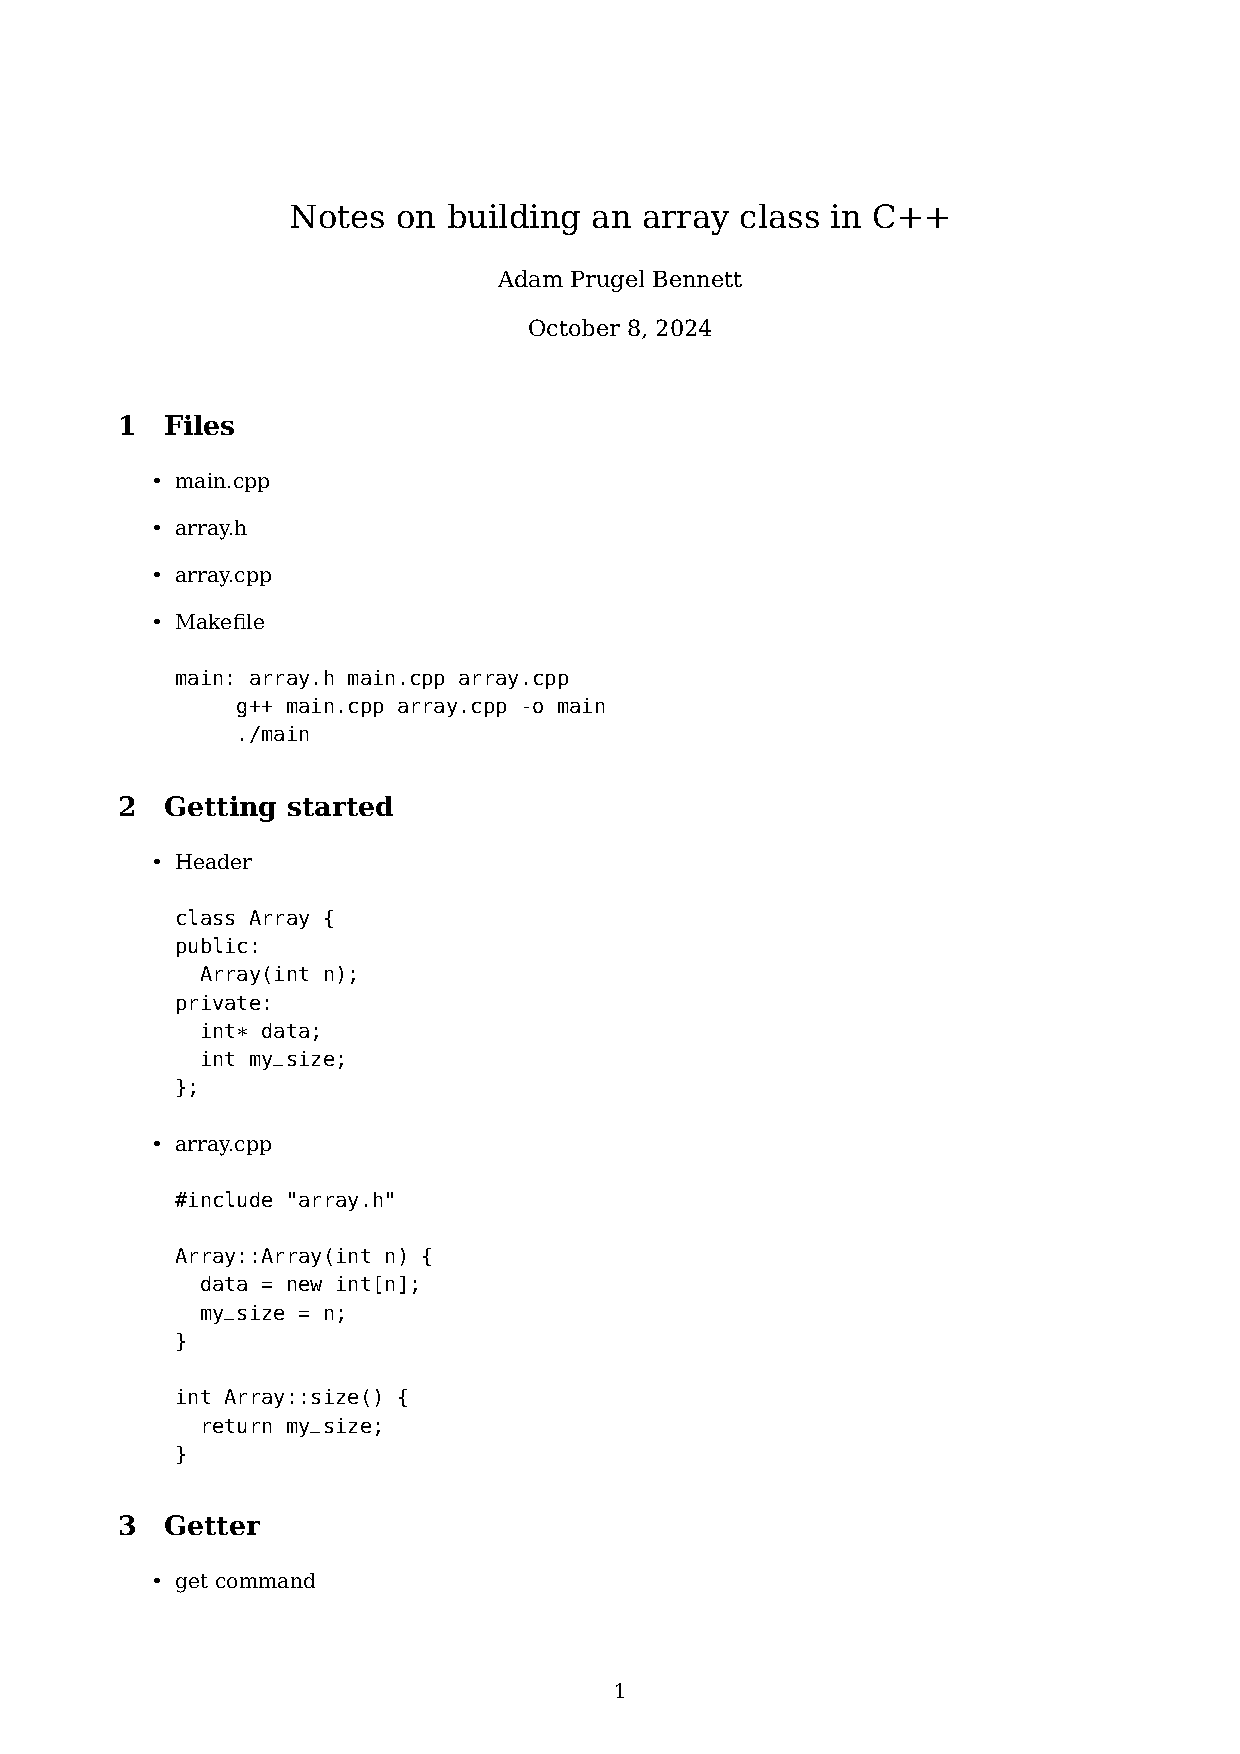
\includegraphics[width=10cm]{array}
\end{minipage}
\end{slide}
\addtocounter{outlineitem}{1}
}

\setcounter{outlineitem}{1}
\Outline
\toptarget{firstoutline}

%%%%%%%%%%%%%%%%%%%%%%% Next Slide %%%%%%%%%%%%%%%%%%%%%%%

\begin{slide}
\section{Use Arrays}

\begin{PauseHighLight}
  \begin{itemize}
  \item An array is a contiguous chunk of memory\pause
  \item In C we can create arrays using\\
    \jl$int *array = new int[20]$\pause
  \item The array has an access time of $\Theta(1)$\pause
  \item The constant factor is small (i.e. access time $\approx 1$ time
    step)\pause
  \item Arrays provide a very efficient use of memory\pause
  \item 95\% of the time using arrays is going to give you the best
    performance\pause, although never use raw arrays!\pauseb
  \end{itemize}
\end{PauseHighLight}
\end{slide}


%%%%%%%%%%%%%%%%%%%%%%% Next Slide %%%%%%%%%%%%%%%%%%%%%%%

\begin{slide}
\section{Disadvantages of Arrays}

\begin{PauseHighLight}
  \begin{itemize}
  \item Arrays have a fixed length\pause
  \item Very often we don't know how big an array we want
    \begin{itemize}
    \item E.g. reading words from a file\pause
    \end{itemize}
  \item Adding or deleting elements from the middle of an array is
    costly\pause
  \item Sorted arrays are expensive to maintain\pause
  \item Arrays don't know how big they are\pause---annoying\pauseb
  \end{itemize}
\end{PauseHighLight}

\end{slide}

%%%%%%%%%%%%%%%%%%%%%%% Next Slide %%%%%%%%%%%%%%%%%%%%%%%
\Outline

%%%%%%%%%%%%%%%%%%%%%%% Next Slide %%%%%%%%%%%%%%%%%%%%%%%

\begin{slide}
\section{Variable Length Arrays}
\toptarget{varover}
\begin{PauseHighLight}
  \begin{itemize}
  \item We want a variable length array\pause
  \item Initially a variable length array would have length zero\pause
  \item We should be able to
    \begin{itemize}
    \item Add an element to an array
    \item Access any element in the array
    \item Change an element
    \item Delete elements
    \item Know how many elements we have\pause
    \end{itemize}
  \end{itemize}
\end{PauseHighLight}
\end{slide}

%%%%%%%%%%%%%%%%%%%%%%% Next Slide %%%%%%%%%%%%%%%%%%%%%%%

\begin{slide}
\section{ADT for a List}

\pausebuild
\begin{itemize}
\item What do we want of a list of \jl$int$s?\pause
  \begin{itemize}
  \item \jl$void push_back(int value)$\pause
  \item random access \jl$array[i]$\pause
  \item \jl$int size()$\pause
  \end{itemize}
\item It would be useful if it resized\pause
\item It would be great to have some algorithms (e.g. sort) that can
  be run on a list\pause
\end{itemize}

\end{slide}

%%%%%%%%%%%%%%%%%%%%%%% Next Slide %%%%%%%%%%%%%%%%%%%%%%%

\begin{slide}
\section{Implementation}

\begin{itemize}
\item How should we implement a list?\pause
\item Use an array, of course!\pause
\item We need to distinguish between
  \begin{itemize}
  \item the number of elements in the list \jl$size()$
  \item the number of elements in the array \jl$capacity()$\pause
  \end{itemize}
\item If the number of elements grows larger than the capacity then we
  need to increase the capacity\pause
\end{itemize}
\end{slide}

%%%%%%%%%%%%%%%%%%%%%%% Next Slide %%%%%%%%%%%%%%%%%%%%%%%

\begin{slide}
\section{Initial Capacity}

\begin{PauseHighLight}
  \begin{itemize}
  \item We could prevent resizing arrays by using a huge initial
    capacity\pause
  \item However, how big is big enough?\pause
  \item What happens when we have an array of arrays?\pause
  \item Memory like time is resource we should care about\pause
  \item In an analogy with \emph{time complexity} we also care about
    \emph{space complexity} (i.e. how much memory we need)\pause
  \item If we want to store $n$ elements it is reasonable to expect that
    we use $c\, n$ bits of memory where we want to keep $c$ small\pause
  \end{itemize}
\end{PauseHighLight}
\end{slide}


%%%%%%%%%%%%%%%%%%%%%%% Next Slide %%%%%%%%%%%%%%%%%%%%%%%

\begin{slide}
\section{Resizing Memory}

\pausebuild
\begin{itemize}
\item We start with some reasonable capacity\pause
\item We can add elements\pause{} \pauselevel{=6}
  until we reach the capacity\pause
\item A simple method for resizing memory is
  \begin{itemize}
  \item create a new array with double the capacity of the old
    array\pause 
  \item copy the existing elements from the old array to the new
    array\pause
  \end{itemize}
\end{itemize}
\begin{center}\pauselevel{=1}
  \multipdf[width=\textwidth]{VariableSizeArray}\pause
\end{center}
\end{slide}


%%%%%%%%%%%%%%%%%%%%%%% Next Slide %%%%%%%%%%%%%%%%%%%%%%%

\begin{slide}
\section{Amortised Time Analysis}
\toptarget{vartime}
\begin{PauseHighLight}
  \begin{itemize}
  \item How efficient is resizing?\pause
  \item Most \jl$push_back(elem)$ operations are $\Theta(1)$\pause
  \item When we are at full capacity we have to copy all elements\pause
  \item Adding to a full array is slow but it is \emph{amortised} by
    other quick adds\pause
    \begin{quote}
      \emph{amortised:} effect of a single operations `deadened' by
      other operations\pause
    \end{quote}
  \end{itemize}
\end{PauseHighLight}

\end{slide}

%%%%%%%%%%%%%%%%%%%%%%% Next Slide %%%%%%%%%%%%%%%%%%%%%%%

\begin{slide}
\section{Example}

\pausebuild
\begin{itemize}
\item If we have an initial capacity of 10 and add 100 elements then the
  number of operations needed is
  \begin{itemize}
  \item adds: 100\pause
  \item copies: 10\pause+20\pause+40\pause+80\pause=150\pauseb
  \item \jl$new int[]$: 4\pause
  \end{itemize}
\item 250 adds and copies operations + 4 \jl$new$ operations\pause
\end{itemize}


\end{slide}

%%%%%%%%%%%%%%%%%%%%%%% Next Slide %%%%%%%%%%%%%%%%%%%%%%%

\begin{slide}
\section[-2]{General Time Analysis}

\begin{itemize}
\item If we perform $N$ adds with an initial capacity of $n$\pause
\item We must perform $m$ copies where
  \begin{center}
    \includegraphics[width=0.9\linewidth]{doubling}
  \end{center}\vspace*{-1cm}
  \begin{align*}
    n\times 2^{m-1} &< N \leq n \times 2^{m}\pause &
    \mbox{i.e.}\quad 
    m = \left\lceil \log_2\left(\strut \frac{N}{n} \right) \right\rceil\pauseb
  \end{align*}
\item The number of elements copied is
  \begin{align*}
    n + 2 n + 4 n + \cdots + 2^{m-1} \, n\pause=n(1 + 2 + \cdots + 2^{m-1})
    \pause = n \, (2^{m}-1)\pause
  \end{align*}
\item Total number of operations is (using $\lceil \log(a) \rceil <
  \log(a) +1$)
  \begin{align*}
    N + n \, (2^{m}-1) \pause= N + n 2^{\left\lceil \log_2\bigl(
      \tfrac{N}{n} \bigr) \right\rceil} -n \pause < N +2 N -n 
    \pause< 3N\pause
\end{align*}
\end{itemize}

\end{slide}

%%%%%%%%%%%%%%%%%%%%%%% Next Slide %%%%%%%%%%%%%%%%%%%%%%%

\begin{slide}
\section{Insertion and Deletion}

\begin{PauseHighLight}
  \begin{itemize}
  \item \jl$vector<T>$ is very useful and very fast for lots of
    things\pause
  \item But if you try to insert or delete an element anywhere other
    than the end then you have to shove all the subsequent elements
    one space forward\pause
  \item This is not the right data structure if you want to keep
    elements in order\pause{} (binary trees will do that for
    you much more efficiently)\pauseb
  \item Linked lists allow you to splice in a sublist into a list in
    constant time\pause{} although linked lists have a lot of
    drawbacks\pauseb
  \end{itemize}
\end{PauseHighLight}

\end{slide}


%%%%%%%%%%%%%%%%%%%%%%% Next Slide %%%%%%%%%%%%%%%%%%%%%%%
\Outline

%%%%%%%%%%%%%%%%%%%%%%% Next Slide %%%%%%%%%%%%%%%%%%%%%%%

\begin{slide}
\section{Computer Languages}
  
\begin{PauseHighLight}
  \begin{itemize}
  \item Different computer languages are designed for different roles
    and have different advantages and disadvantages\pause
  \item \emph{C++} was designed to be fast (as fast as C)\pause, it
    pays the price of allowing bugs that hard to detect\pauseb
  \item \emph{Java} was designed to be vary safe (avoiding lots of
    bugs)\pause, but is not fast and a bit long winded\pauseb
  \item \emph{Python} was designed so you can rapidly write powerful
    programmes with a small amount of code\pause, but it is not fast
    or safe\pauseb
  \end{itemize}
\end{PauseHighLight}

\end{slide}

%%%%%%%%%%%%%%%%%%%%%%% Next Slide %%%%%%%%%%%%%%%%%%%%%%%

\begin{slide}
\section{Problems with C++}
  
\begin{PauseHighLight}
  \begin{itemize}
  \item Amongst a number of issues that make C++ dangerous are
    \begin{itemize}\squeeze
    \item Memory management
    \item Writing to parts of memory that you should not
    \item Multiple inheritance\pause, although you seldom need to do this\pauseb
    \end{itemize}
  \item However, by using existing data structures (STL) and following
    established programming patterns these don't have to be an issue\pause
  \end{itemize}
\end{PauseHighLight}

\end{slide}

%%%%%%%%%%%%%%%%%%%%%%% Next Slide %%%%%%%%%%%%%%%%%%%%%%%

\begin{slide}
\section{Memory Management}

\begin{PauseHighLight}
  \begin{itemize}
  \item Most programming languages have two types of memory
    \begin{description}
    \item[The Stack:] is the area of memory controlled by compiler for
      local variables, function calls, etc.\pause
    \item[The Heap:] is area that the programmer (you) can
      request\pause, which is nice\pauseb
    \end{description}
  \item In C++ you are given the \emph{right} to ask for memory
    \begin{cpp}
      int *storage = new int[n];
    \end{cpp}\pauseb
  \item You have \emph{responsibility} to free the memory
    \begin{cpp}
      delete[] storage;
    \end{cpp}\pauseb
  \end{itemize}
\end{PauseHighLight}

\end{slide}

%%%%%%%%%%%%%%%%%%%%%%% Next Slide %%%%%%%%%%%%%%%%%%%%%%%

\begin{slide}
\section[-2]{Trouble with Memory Management}

\begin{PauseHighLight}
  \begin{itemize}
  \item If you don't release memory acquired with \texttt{new} using
    \texttt{delete} you cause a \emph{memory leak}\pause
  \item Often memory leaks are no concern, but in large programs
    memory leaks will rapid exhaust the computer's memory, slowing
    down the code and eventually leading to the programme
    crashing\pause
  \item To release a block of memory we can use: \jl$delete[] storage;$\pause
  \item Now \texttt{storage} is a \emph{dangling pointer} and must not
    be used as it is no longer valid\pause
  \item If we accidentally delete the storage twice we get an
    \textit{undefined behaviour}\pause, but often the programme will crash\pause
  \end{itemize}
\end{PauseHighLight}

\end{slide}



%%%%%%%%%%%%%%%%%%%%%%% Next Slide %%%%%%%%%%%%%%%%%%%%%%%

\begin{slide}
\section{Resource Acquistion is Initialisation (RAII)}

\begin{PauseHighLight}
  \begin{itemize}
  \item Java and Python use garbage collectors which automatically
    checks whether memory can be accessed and if not it is
    removed\pause
  \item In C++ this is your responsibility\pause
  \item But there is a standard \emph{programming pattern} to elevate
    the problem known as \emph{Resource Acquistion is Initialisation
      (RAII)}\pause
    \begin{quote}
      \it Wrap all resources in classes.  Request the resources in the
      constructor and release the resource in the destructor\pause
    \end{quote}
  \item When the object goes out of scope (you leave a \texttt{for}
    loop, function call, etc.) the destructor is called and the
    resource is safely released\pause
  \end{itemize}
\end{PauseHighLight}

\end{slide}

%%%%%%%%%%%%%%%%%%%%%%% Next Slide %%%%%%%%%%%%%%%%%%%%%%%

\begin{slide}
\section{RAII}

\begin{PauseHighLight}
\begin{cpp}
  template <typename T>
  class container {
    private:
      T* data;
    
    public:
      container(unsigned n) {data = new T[n];}$\pause$
      ~container(unsigned n) {delete[] data;} $\pauselevel{=3}\pauseb$
  };$\pauselevel{=1}\pause$

    
    main() {

      for (int i=0; i<1000; ++i) {
        container<int> my_container(10000);
        // $do something$
      }

    }$\pause$
\end{cpp}

\end{PauseHighLight}

\end{slide}


%%%%%%%%%%%%%%%%%%%%%%% Next Slide %%%%%%%%%%%%%%%%%%%%%%%

\begin{slide}
\section[-2]{Writing over Memory}

\begin{PauseHighLight}
  \begin{itemize}
  \item In C++ the following will compile and run
    \begin{cpp}
      int *array = new int[4];
      int *a = new int[2];
      double *darray = new double[4];
      array[4] = 4;
    \end{cpp}\pause
    \vspace*{-1cm}
  \item However \jl$array[4]$ has not been assigned (unlike
    \jl$array[0]$, \jl$array[1]$, \jl$array[2]$ and \jl$array[3]$)\pause
  \item The memory on the heap corresponding to the address of
    \jl$array[4]$ might have been assigned to \jl$a[0]$ in which case
    you may inadvertently have set \jl$a[0]$ to 4 leading to the
    program not doing what you want\pause
  \item It might be that you have put an \texttt{int} into
    \jl$darray[0]$ which will then crash the system when you read
    \jl$darray[0]$\pause
  \end{itemize}
\end{PauseHighLight}

\end{slide}

%%%%%%%%%%%%%%%%%%%%%%% Next Slide %%%%%%%%%%%%%%%%%%%%%%%

\begin{slide}
\section{Guarding Against Mistakes}

\begin{PauseHighLight}
  \begin{itemize}
  \item These are really hard problems to debug because where the
    program goes wrong or crashes can be very far from the assignment
    that caused the error\pause
  \item Java takes the approach that it always tests whether you are
    writing in valid memory\pause
  \item By default C++ doesn't even for data structures\pause---making
    this check slows down random access\pause
  \item Checks can also make pipeline optimisations harder to
    make\pause
  \item The onus is on the user to use the memory correctly\pause
   \end{itemize}
\end{PauseHighLight}

\end{slide}

%%%%%%%%%%%%%%%%%%%%%%% Next Slide %%%%%%%%%%%%%%%%%%%%%%%

\begin{slide}
\section{Follow Programming Idioms}

\begin{PauseHighLight}
  \begin{itemize}
  \item Using common data structures and following common idioms will
    prevent most errors
  \end{itemize}
  \begin{cpp}
    int n = 5;
    vector<int> array(n);
    
    for(int i=0; i<array.size(); ++i) {
      array[i] = i;
    }$\pause$

    for(auto pt=array.begin(); pt != array.end(); ++pt){
      *pt *= 2
    }$\pause$
      
    for(int& element: array) {
      element += 2;
    }
  \end{cpp}\pause

  
\end{PauseHighLight}

\end{slide}


%%%%%%%%%%%%%%%%%%%%%%% Next Slide %%%%%%%%%%%%%%%%%%%%%%%
\Outline

%%%%%%%%%%%%%%%%%%%%%%% Next Slide %%%%%%%%%%%%%%%%%%%%%%%

\begin{slide}
\section{Stacks}

\begin{PauseHighLight}
  \begin{itemize}
  \item Lets look at implementing a stack\pause
  \item Remember a stack has methods
    \begin{itemize}
    \item \jl$push(Object )$
    \item \jl$pop()$
    \item \jl$top()$
    \item \jl$empty()$\pause
    \end{itemize}
\end{itemize}
\end{PauseHighLight}
\end{slide}

%%%%%%%%%%%%%%%%%%%%%%% Next Slide %%%%%%%%%%%%%%%%%%%%%%%

\begin{slide}
\section[-1]{Implementation of Stack}

\begin{cpp}
template <typename T>
class MyStack
{
private:
  std::vector<T> stack;$\pause$

public:
  void push(const T& obj) {stack.push_back(obj);}$\pause$

  T top() const {return stack.back();}$\pause$

  T pop() {
    T tmp = stack.back();
    stack.pop_back();
    return tmp;
  }$\pause$

  T empty() {return stack.size()==0;}$\pause$
};
\end{cpp}
\end{slide}

%%%%%%%%%%%%%%%%%%%%%%% Next Slide %%%%%%%%%%%%%%%%%%%%%%%

\begin{slide}
\section[-1]{Notes on Implementation}

\begin{PauseHighLight}
  \begin{itemize}
  \item I don't need to write a constructor as C++ generates a default
    constructor that will initialise the stack correctly\pause
  \item I don't need to write a desctuctor because by default the
    destructor for \jl$vector<T>$ will be called which releases
    memory\pause
  \item I've written the \texttt{pop} command, that I like, but if I
    run
    \begin{cpp}
      stack<Widget> widget_stack;
      Widget w;
      widget_stack.push(w);
      Widget w1(widget.pop());
    \end{cpp}
    if the last command throws an exception then the last term on the
    stack is lost for ever\pause
  \end{itemize}
\end{PauseHighLight}

\end{slide}

%%%%%%%%%%%%%%%%%%%%%%% Next Slide %%%%%%%%%%%%%%%%%%%%%%%

\begin{slide}
\section[-2]{Why not use a \texttt{vector}}
  
\begin{PauseHighLight}
  \begin{itemize}
  \item Surely it is mad to use \jl$MyStack<T>$ as I could just use
    the more powerful \jl$vector<T>$\pause
  \item I can make \jl$MyStack<T>$ as efficient as \jl$vector<T>$ by
    inlining function calls\pause
  \item But why would I want to lose functional?\pause
  \item By using \jl$MyStack<T>$ I am \emph{declaring my intention} of using
    this data structure as a stack\pause
  \item I'm not going to do something weird like modify an element
    inside the stack\pause
  \item My code becomes self-explanatory\pause---I don't need to write
    comments as it is clear what I am doing\pauseb
  \end{itemize}
\end{PauseHighLight}

\end{slide}


%%%%%%%%%%%%%%%%%%%%%%% Next Slide %%%%%%%%%%%%%%%%%%%%%%%

\begin{slide}
\section{Using \texttt{MyStack}}
\pb

  \begin{itemize}
  \item Implementing a stack using a dynamically re-sizable array is
    trivial\pause
  \item Stacks have many applications\pause
  \item E.g. suppose we want to write a program to reverse the order of
    strings in a file\pause
\begin{center}
  \includegraphics[width=\linewidth]{stack-rev0}\mypl{4}
  \multido{\ia=1+1,\ib=5+1}{14}{%
    \llap{\includegraphics[width=\linewidth]{stack-rev\ia}}\mypl{\ib}}
\end{center}

  \end{itemize}

\end{slide}


%%%%%%%%%%%%%%%%%%%%%%% Next Slide %%%%%%%%%%%%%%%%%%%%%%%

\begin{slide}
\section[-1]{Reversing Strings in File}

\begin{cpp}
#include <stack>
#include <iostream>
#include <fstream>
using namespace std;

int main(int argc, char *argv[]) {
  ifstream in(argv[1]);

  stack<string> stack;

  string word;
  while (in >> word)
    stack.push(word);

  while(!stack.empty()) {
      cout << stack.top() << ' ';
      stack.pop();
  }
}
\end{cpp}
\end{slide}

%%%%%%%%%%%%%%%%%%%%%%% Next Slide %%%%%%%%%%%%%%%%%%%%%%%

\begin{slide}
\section{Lessons}

\begin{PauseHighLight}
  \begin{itemize}
  \item Arrays are very efficient both in space (memory) and access
    time\pause
  \item Resizing an array is not that costly\pause
  \item insertion and deletion are expensive, $O(n)$\pause
  \item Arrays are often the simplest way to implement many other
    data structures, e.g. stacks\pause
  \item Use (dynamically re-sizable) arrays (\jl+vector<T>+)
    frequently!\pause
  \item Stop using raw arrays\pauseb
  \end{itemize}
\end{PauseHighLight}

\end{slide}
